\documentclass[sheet]{GL2020}

\usepackage{graphicx}
\graphicspath{ {./images/} }
\usepackage{xcolor}
\usepackage{hyperref}
\usepackage{multicol}
\usepackage{ltablex}
\usepackage{tabularx}
\usepackage{makecell}
\usepackage{indentfirst}
\renewcommand{\tabularxcolumn}[1]{m{#1}}
\setlength{\columnsep}{1cm}

%% document-wide tweaks
\interlinepenalty10000
\setstretch{1}
\def\mytype{Rules and Scenario}
\lfoot{}\rfoot{}

\begin{document}

%% layout for cover page
\thispagestyle{empty}
\parskip0pt

%% title box
\begin{center}\LARGE\bf\begin{tabular}{|c|}
 \hline \gamename\\ \gamedate\\ Rules and Scenario\\ \hline
\end{tabular}\end{center}

\vfill\vfill

This game and all materials thereof are copyright 2021 by Acata Felton, Aaron Sunshine, Eric Fritz, Jeremy Cole, Kelsey Miranda, and Koh Henderson. Additions and updates have been made for the 2024 run by Acata Felton, Aaron Sunshine, Kit Hill, and Olivia Montoya. We also want to credit the MIT Assassins' Guild for the origin of many of the base rules used in this game.\\

\vfill\vfill

\begin{center}\bf
 BROUGHT TO YOU BY THE LUMINARY ROLEPLAY SOCIETY
\end{center}

\vfill

\clearpage

%% layout for Table of Contents page
\thispagestyle{empty}
\tableofcontents

\clearpage

%% layout for main body of rules
\setcounter{page}{1}
\parskip5pt
\vfill
\section{Introduction}

The following are the rules for {\em\gamename}, a real-time, real-space, roleplaying game sponsored by the Luminary Roleplay Society. \textcolor{red}{This version of the rules has been updated as of 20Sep2024. Changes, additions, and clarifications are presented in red text, just like this.}

\subsection{Expectations for Players}
You are responsible for knowing and following these rules. It is through the constraints created by these rules and other mechanics that the intended play experience is made possible. Many of these rules are nigh-impossible for GMs to enforce, and rely upon the honor system. Do not cheat. Do not abuse loopholes. Play fair. To do otherwise will deprive both yourself and your fellow players of the experience you signed up for.

We estimate the number of pages of reading for this game is between 40 and 50 pages for most characters, but this may change a little as we finalize game material. This page estimate is across all of the documents, including this rules document. Please make sure you set aside enough time to prepare for game by familiarizing yourself with all of the documents. You do not need to memorize anything (except maybe your CR stat), but you should read everything in detail at least once, and know where to look up information. \textbf{Print copies of everything will be provided at game.}

\subsection{GM Commitment}
The \textbf{gamemasters} (\textbf{GMs}) run the game. If you have any problems or questions concerning the game, contact a GM. Rulings the GMs make are final. They may violate the letter of the rules to preserve the spirit. The GMs promise to be as fair and reasonable as possible. Neither they nor these rules are perfect, so we ask for your understanding and flexibility. Your GMs for this game are: Acata Felton, Aaron Sunshine, Kit Hill, and Olivia Montoya.



\section{Logistics}
\subsection{Basic Information}
\begin{itemize}
 \item \textbf{Dates and Times:} Players will be expected to be on site at the event location from 12 pm on Fri, Oct 4th - 5 pm on Sun, Oct 6th. Arriving late or leaving early requires special dispensation from the GMs. Please request any such arrangements well in advance.
 \item \textbf{Location:} Silver Lake Conference Center; 223 Low Road Sharon, CT 06069. (Approx. 3 hr 15 min drive from BOS Airport, 2 hr 15 min from JFK Airport, or 1 hr 30 min from Albany or Bradley Airports.)
\end{itemize}

\section{Game Content}
As this is a S\&P game, the GM team has prepared extensive information about the premise and direction of the game, as well as the types of personal plots and stories that are likely to show up. Please see the Design Document for extensive details.

\subsection{The Premise}
\emph{Welcome to the world of \pEarth{}. The Gods have gifted the people with magic, helping them to survive the ravages of a devastating magical Storm that roams across the continent once every 3 years. Only a chosen few students can manipulate the path of these magical Storms. Until recently, a treaty ensured a tenuous peace. The three nations agreed that the Storm should hit each nation in turn, sharing the devastating burden. Although the Storms always took their toll, no one nation suffered too greatly. That all changed when the treaty was broken, and a nation betrayed. Although their architects and diplomats struggle to repair what was lost, the work won't be complete by the next Time of Deciding.}

\emph{Our story begins at the center of the known world. Here at the \pSchool{}, students are trained in the rituals necessary to change the path of the Storm. Instructors maintain the veneer of impartiality — but in reality, each fights for their own nation's interests to varying degrees, all vying for control of the magical disaster. But despite their efforts, no nation has the complete picture — and new interests conspire to change the fate of the world. Where the magic will ravage next — and what consequences it will have — are for you to decide.}


\section{Safety}
This is only a game. Everyone involved should act with courtesy, sportsmanship, patience, and taste. The GMs may expel anyone they believe to be violating the spirit of the rules or the game. Emotions may run high. If you think things are crossing the line from game to reality too much, or if you are just getting too stressed, take a break. Always, play safely, then play to have fun. 

Real violence is unacceptable. Game action should cause no real-world damage, either to people or property. If something dangerous is happening, call a halt. Stay in control, use common sense, and do not endanger yourself or others.

Safety is a shared responsibility in the community, between all of the participants, players and GM alike. Only you can determine if you need to step away from a scene, plot, player, etc. Only you can say whether you need a temporary or a permanent solution. But we can all be aware of the ways that we interact with others, and be willing to adjust our behavior based on feedback for the safety and comfort of our fellow participants.


\subsection{Calibration}
\textbf{Players are more important than the game.} In this game, this adage must be applied preemptively, not just when someone gets activated or upset in the middle of game. Secrets and Powers games can survive a character not being present, but the game is the poorer for it. This is due to the design concept that any character the game could run without should either be cut before casting, or rewritten to be more integral. This makes it way less likely that a player will be bored or feel left out, but it does pose important considerations for safety. Due to this, we ask that you take care of yourself and check in regularly with yourself before the game (making sure that the character does not have content that you are concerned about or feel uncomfortable playing) and during the game (so you can come speak to the GMs if need be during game). However, if you do need to leave the game for an extended period of time for whatever reason, we will make it work. You are more important than this game.

Calibration is handled primarily through casting.We ask you to read over it and let us know \textbf{as soon as possible} if there are aspects we need to change. Please don't just change things on your own without talking to the GMs; we need to re-balance game around the changes.

\subsubsection{Expectation Management}
You may find it a valuable exercise to take a few minutes \textbf{before} arriving at the event to ask yourself: What do you as a player hope to get out of this experience? What would constitute a successful or worthwhile event to you? Are there any experiences you wish to avoid, or patterns from previous games you wish to challenge? What actions can you take to help with these things?

\subsubsection{Player to Player Calibration}
This game style generally relies on little to no player to player calibration. Characters are written to fall within the comfort levels indicated on casting surveys given most likely interactions with other characters. In situations where calibration is necessary, it should be accomplished in character if possible. If not possible, then the OOC calibration should be kept as short as possible. We want to allow as much as possible to unfold organically in game.

While calibration for how you want play to proceed in terms of steering and plot should follow the rules above, we encourage stepping out of game if you find yourself unable to continue with a scene or a situation for your own personal safety and well being. If you feel comfortable, speaking with a player out of game about what you need for the scene or content to continue is an important form of OOC collaboration that is often challenging to do while still in character. In these situations, please step out of character and take the time you need. If what you need is some time out of game, please let a GM know so we can help other characters who may be looking for you. If you need help re-engaging or have other concerns, please do come see a GM or your NPC, \cPrincipal{}.

If you wish to do any pre-play calibration at dinner on Friday night, first ask ``are you open to pre-game calibration with me?'' without further detail. Remember that other players may not be aware that they have a plot with your character, may not believe calibration is necessary (IC or OOC), or may prefer to go in without expectations. In such a case, respect your fellow players' choices and contact a GM if you want support for yourself.

\subsubsection{Negotiating Outcomes and Pre-Planning}
This game style \textbf{does not support} negotiating outcomes or pre-planning. These games are very much ``play to discover'' and scheduling reveals, scenes, or activities limits that spontaneity and creates closed circles that other players cannot breach. In this, we very much ask players to ``trust the process'' and act like your character would act. Trust that your fellow players will respond in interesting ways that will enrich your story without you needing to know what that reaction is ahead of time.

The exception to this is if you as a player want to plan an event that is open to other characters that is not plot related but instead a space for folks to gather for plot to happen. If you do want to do this, please still let a GM know before the game so we can help schedule space and time or let you know if it needs to be changed in any way. This is absolutely not necessary and this game has plenty to do without players needing to create events. However, we do know that this type of planning is something that some players like to do. For example, if a student wanted to have a student party on Friday night to help students relax before all the big decisions, that type of event would be welcome.

\subsubsection{Self Care}
\textbf{Players are more important than the game.} Take some time in the days or weeks leading up to game to ask yourself what you need to take care of yourself. We want you to have the best chance of having an enjoyable experience at game, and contingencies in case that doesn't happen. Reflect on the game scenario and the listed content warnings (see the Design Document). Reflect on your mental, physical, and emotional reserves, and what actions you can take to prepare care for yourself before game to boost your resiliency. Review the safety mechanics (see below) for this game. It is also a good idea to be prepared in case of drop or bleed afterward. See the ``Post Game Workshops'’ section below for more information about these terms.

We have a culture of care for others in this game, as seen below in our safety mechanics. However, no one can read minds, and it is up to every player to self advocate if they need something changed (either with GMs or their fellow player). This also means recognizing when something may be too upsetting or hard to deal with for you as a player and exciting the scene to take care of yourself. We provide mechanics for doing this below. 

\subsection{Safety Mechanics}
When in doubt, use the universal Out of Game symbol of placing a fist on top of your head. Use this to go out of character and talk, or do whatever you need to as players to re-establish a safe play space, or address an out of character situation. 

Your GMs will be available during game to assist and facilitate as well. During game on hours, we will either have someone available at GM Headquarters, or leave a note with where to find us. We are not trained mediators or therapists, but we care about you and want you to have a good time. We can help you come up with plans for self comforting, and when you are ready, help you decide if and how you want to re-engage with game.

The following safety mechanics will be used in ``\gamename{}''. These are for player safety. Deliberately ignoring another player's use of them will have disciplinary consequences. You may \textbf{not} use these safety mechanics to avoid in game consequences for character actions.

\begin{tabularx}{\textwidth}{| m{4cm} | X |}
\hline
	\multicolumn{2}{|c|}{\textbf{Out of Game / Out of Character (OOC) Hand Signal}}\\
\hline
	\textbf{How to Use:} Make a fist with one hand. Place it on top of your head (visible from in front of and behind you) & \textbf{\newline What Happens:} You are now out of character (OOC). You may talk and act as your player. This is useful for many things including talking player to player about something that just happened that you need to adjust, stepping out to use the restroom, or because a mechanic told you to. \newline\newline This is the main way we ask you to do calibration, including addressing something that needs to change in a scene for your safety or if you need to de-escalate a scene that has become too intense for any reason. If you are requested by a player to tone it down or change something for their safety and comfort, that is not a request. You must de-escalate. \newline\newline If someone uses this around you, your character no longer sees theirs. You should ignore OOC players unless they address you directly and ask you to go OOC too to discuss something. If you need to have an extended conversation OOC, we encourage you to step away from ongoing game play so as not to disrupt it. \newline \\
\hline
	\multicolumn{2}{| p{16cm} |}{\textbf{\newline Example:} \newline Players 1 and 2 are playing an intense scene. As their character, Player 2 accuses Player 1's character of keeping a secret from them and begins to yell. Player 1 realizes that they are feeling trapped and this is too much for them at the moment. They raise the OOC sign, which stops the scene.\newline Player 1: I need you to de-escalate the scene. I am feeling pretty overwhelmed.\newline Player 2: What can I do to help?\newline Player 1: I need a bit of space and a moment. Then could we continue this without as much yelling and with more distance between us?\newline Player 2: Of course! Let me know when you are ready. I will go get a drink of water in the meantime. \newline}\\
\hline
\hline
	\multicolumn{2}{|c|}{\textbf{The Okay Check In}}\\
\hline
	\textbf{\newline How to Use:} Make eye contact with the person you want to check with, and flash them the ``ok'' symbol with your hand. They should respond with a ``thumbs up,'' ``thumbs down,'' or ``thumbs sideways'' \newline & \textbf{What Happens:} Use this mechanic to check in with someone who appears to be in distress (e.g.: crying), whose demeanor has suddenly changed (e.g.: stopped talking and has a 50-yard stare), or you otherwise want to check in on whether the \textbf{player} under the character is doing okay. If you get a ``thumbs down'’ or ``thumbs sideways'’ response, pause game play and take a moment out of character to check in with the player. Encourage them to check in with themselves if they need to change anything about current play or the current environment. If you don't feel able to check in with them at that time, find a GM or send them to GM HQ. \\
\hline
	\multicolumn{2}{| p{16cm} |}{\textbf{\newline Example 1:} \newline Player 1 walks into a room and sees Player 2 sitting in a corner crying while two other players are debating something intensely in character. Player 1 catches Player 2’s eye and makes the okay sign at them. Player 2 gives them the thumbs up and then goes back to crying. Player 1 continues on their way, knowing that Player 2 was having a good in character cry. \newline}\\
\hline
	\multicolumn{2}{| p{16cm} |}{\textbf{\newline Example 2:} \newline Player 1 walks into a room and sees Player 2 sitting in a corner crying while two other players are debating something intensely in character. Player 1 catches Player 2’s eye and makes the okay sign at them. Player 2 gives a thumbs sideways. Player 1 makes the OOC sign and goes over to them.\newline Player 1: Is there any way I can support you right now?\newline Player 2: I am feeling like no one wants to talk to me and I don’t know what to do.\newline Player 1: Do you want to talk about it or maybe go talk to a GM?\newline Player 2: Yeah, I think I need to talk to a GM.\newline Player 1: Okay, would you like me to come with you?\newline Player 2: That would be great, thanks. \newline}\\
\hline
\hline
	\multicolumn{2}{|c|}{\textbf{Game Halt}}\\
\hline
	\textbf{\newline How to Use:} Say ``Game Halt'' in a loud enough voice for people right around the corner to hear you, but not so loud as to shout. End the halt once the issue is resolved by saying ``3, 2, 1, Game On''. \newline & \textbf{What Happens:} This call should be used to halt game play in a wide area, to sort out a safety issue and everyone in a scene needs to be involved. This includes a player being unable to continue at the moment, a need for calibration, or physical danger. This call is also used by some mechanics to pause the game to fetch a GM for something. Use this call sparingly and use the OOC symbol instead when possible. \\
\hline
	\multicolumn{2}{| p{16cm} |}{\textbf{\newline Example 1:} \newline Player 1 is backing away from an angry mob of characters, and getting dangerously close to a staircase. Player 2 calls ``Game Halt'' and has the group reposition so that Player 1 is no longer in danger of falling. Player 2 then calls ``3, 2, 1, Game on,'' and the scene continues. \newline}\\
\hline
	\multicolumn{2}{| p{16cm} |}{\textbf{\newline Example 2:} \newline There is a large group having a discussion of where the storm should go, and things are getting heated and loud, and everyone is in a small space. Player 1 realizes they are getting deeply overstimulated and that it is hard for anyone to follow the conversation. They also realize they are kind of trapped in a corner in the small space and don’t see a good way to exit. Player 1 calls ``Game Halt!'' At that point everyone should stop and pause the scene.\newline\newline Player 1: Hey all the volume is getting really loud and folks are having a hard time getting words in edgewise. The room is also really crowded. Do you think we could all resume in a larger space and at a lower volume?\newline\newline The group moves to a larger area, and restarts the conversation with less yelling (even if characters are still upset and the scene is really intense) and more attention to sharing the spotlight (maybe not ``realistic,'' but sharing space in game is important for everyone to be able to enjoy themselves). \newline}\\
\hline
\hline
	\multicolumn{2}{|c|}{\textbf{Badge Off}}\\
\hline
	\textbf{How to Use:} At a time when you are not in the middle of a game action, simply take your badge off. & \textbf{\newline What Happens:} Use this to indicate that you are exiting game for the night, or need to take an extended break from game (longer that would be comfortable to maintain the Out of Game Hand Signal). If you are going ``Badge Off'’ for a game related reason, feel free to come find a GM if we can be of any help. Players should assume that another player without their badge is out of character for an extended period. You may take no game actions toward someone who isn't wearing their character badge. If you are looking for their character, assume they cannot be found. \newline \\
\hline
\hline
	\multicolumn{2}{|c|}{\textbf{Open Door Policy}}\\
\hline
	\textbf{How to Use:} Physically leave the game space. & \textbf{\newline What Happens:} If you need to leave the game space (e.g.: returning to your room, or leaving the venue), please do so. If you leave, PLEASE, let a GM know so we don't start a search and rescue operation assuming you are lost in the woods somewhere. \newline \\
\hline
\end{tabularx}

\section{Game Schedule}
The full game schedule and site map are provided in a separate greensheet. 

\paragraph{Pre-Game Workshops:} There will be a series of \textbf{mandatory} pre-game workshops on Friday afternoon to help with building player rapport and establishing the shared contract of the game.

\paragraph{Mid-Game Reflection:} There will be an \textbf{optional} OOC activity offered over dinner on Saturday to recalibrate and redirect to improve your play experience.

\paragraph{Post Game Workshops:} Formal derole and debrief are optional, but highly encouraged activities after the game ends. These activities help with \textbf{bleed}: character feelings affecting player experiences, in this case after the game (i.e.: a player is short with someone at work after an intense weekend game). These activities also help with \textbf{drop}: players feeling low emotions after interacting closely with people for several days and then going their separate ways.

\section{Getting Started}
\subsection{Unless You Know Otherwise}
You will see the term ``unless you know otherwise'' scattered throughout this document and many other game documents. This phrase is a common shorthand that means the general rules as written preclude something, but that does not mean that this thing is impossible. For example, some characters may have a greensheet, ability, or a character stat that allows them to do something that normal people can't. Ask a GM if you are not sure whether something you have qualifies to allow you to bypass an ``unless you know otherwise.''

\subsection{Character Packets}

Your character packet is a big manila envelope. It contains your role: who you are, what you're trying to accomplish; everything about your part as a {\bf player-character} ({\bf PC}) in the game. Read all the contents and generally keep them with you during the game.If you are missing something or find something which doesn't seem to belong to you, tell one of the GMs. Character packets are confidential. Game materials which cannot be given to other players are marked ``Not Transferable,'' whereas things which can be given to others are marked ``Freely Transferable'' or ``Game Item.'' Do not show ``Not Transferable'' documents to other players; you are always free to share the information through in-character roleplay once the game begins.

Your Character Packet will contain:
\paragraph{Name-Badge:} You will have 2 name badges, one with your Character Name for in game activities, and a second with your Player name for out of game activities. Your IC name-badge will have your character name, pronouns, a brief character description, and {\bf badge number} on it. Wearing this shows that you are in the game; wear it visibly. GMs will provide lanyards to borrow. Your character badge also represents your character's body in-game. Badge numbers are not in-game information. See the \emph{Character Bodies} and \emph{Badge Numbers} sections for more details.

\paragraph{Character Sheet:} Your character sheet describes who you are and what you are up to. It contains a list of everything else that should be in your character packet. \textbf{Do not show or read your character sheet to other players.}

\paragraph{Bluesheets:} A bluesheet describes information common to members of a group. When in conflict, character sheet information overrides bluesheet information. \textbf{Do not show or read a bluesheet to other players.}

\paragraph{Greensheets:} A greensheet describes and expands abilities, mechanics, or in-game knowledge.\textbf{ Do not show or read a greensheet to other players unless a greensheet specifically says that that character has also received that greensheet.}

\paragraph{Stat Card:} Your stat card lists your statistics, and is printed on pink or salmon colored paper. \textbf{Do not show or read your stats to other players}. The reverse side is a {\bf death report}; fill it out and give it to the GMs if your character dies.

The following stats exist in this game:
\begin{enumerate}
	\item Combat Rating (CR) - everyone has a CR. See details below in ``Violence, Death, and Damage.’’
	\item L-Stat - Represents your familiarity with navigating the Library at the \pSc{}.
	\item V-Score - everyone has a V-score. The default is 0. Most players will NOT know what this means, and may not learn during play. Ignore it unless a mechanic asks you to check or change your score. This may not cause you to learn IC or OOC what the score means.
	\item S-Score - everyone has an S-score. The default is 0. Most players will NOT know what this means, and may not learn during play. Ignore it unless a mechanic asks you to check or change your score. This may not cause you to learn IC or OOC what the score means.
\end{enumerate}

\paragraph{Ability Cards:} An ability card explains a special ability your character has, and is printed on yellow paper. The front side (says ``Ability effect'’) describes the effects; show this side to players when you use the ability. The reverse is the rules of use. \textbf{Do not show this side to other players.}

\paragraph{Memory/Event Packets:} A memory packet is an envelope or taped/glued/stapled piece of paper with a {\bf trigger} which describes when to open and read it. If the trigger is a number, open the packet when you see something with that number. If it's a quoted phrase, open when you hear or read it in-game. If it's a symbol, open when instructed. Do not take game action based on an unopened trigger. \textbf{Do not show or read a memory packet to other players.}

\paragraph{Research Notebooks:} A research notebook is a little booklet of pages folded over and stapled shut. These packets guide you through creating or researching something taking many steps, in which the full process that will be required is not known at the start. \textbf{Open the first page when you receive your packet. They will prompt you to open the second page when game starts}. Each page will describe information you learn, and tell you what action to take next. When you complete the requested action, you may open the next page. \textbf{Do not read a research notebook to other players unless you are instructed to do so in the text of the research notebook.}

\emph{Exception:} Some research notebooks will list other characters as having the same notebook. In these cases, if the \textbf{characters} elect to share information, players may open pages to match. I.e.: If Player 1 has opened page 3, but Player 2 has not, after conferring in character and agreeing to share information, Player 2 may open pages up to and including page 3.

\paragraph{Items:} In-game items may be transferred from character to character, and should be marked as such. See the \emph{Items Etc.} section for more details.

\paragraph{Whitesheets:} These are in-game items that are the size of a full piece of paper and represent things like documents and letters with specific content. Treated exactly like any other item.

%% Some Game Fundamentals 
\subsection{Game Concepts}

\paragraph{Not-Here:} Some mechanics may instruct you to go ``Not-Here.'’ You go not-here by turning your name-badge around so the ``I'm Not Here'' side is showing. Putting a hand on your head, visible from a distance, helps if you're near other players. When you are not-here, your character is not there. Your character cannot see, hear, or remember any game actions or information you (the player) happen to encounter. Avoid other characters, common game areas, game signs, or any sort of game interaction. Going ``Not-Here'' is a game mechanic. Doing so in front of other characters represents something like suddenly becoming invisible, and is distinct from the safety mechanics described above.

\paragraph{Player Characters (PCs):} Each player is playing one character. These characters are the PCs.

\paragraph{Non Player Characters (NPCs):} This game has one embedded NPC: \cPrincipal{\intro}. \cPrincipal{\They} \cPrincipal{\are} available both IC and OOC to provide support and guidance for characters and players. Players are always also welcome to come to a GM.

\paragraph{Non-Players:} Use tact and common sense when dealing with non-players ({\bf NPs}). Camp staff have their own lives, and other groups at the camp have their own events to attend. NPs may not knowingly affect the game. They and their rooms may not be used to hold items or information.

Avoid conspicuous or threatening game actions in front of NPs. Please keep conversations about murdering another character and other potentially triggering or upsetting topics out of earshot of NPs. Do \textbf{NOT} shout ``fire'' unless there is a real life, actual fire, or ``he’s got a gun’’ unless there is a real life, actual gun. If there is an in-game danger, you may use stage whispers. If, despite your most valiant efforts, some NPs do get upset, call the GMs who will help calm them down.

If you are about to take an action that would likely upset a nearby NP, you may call a game-halt and relocate the scene. This is considered an out-of-game issue.

\paragraph{Mechanics:} Many actions your character can take, such as walking, talking, and general interaction with other characters, are represented by you doing them. Others, like combat, are performed via abstract mechanics, which are described in ability cards, greensheets, and rules. The abstract information for mechanics (like badge numbers) may not be discussed in-game. If you want to do something special for which there is no mechanic, ask a GM.

Become familiar with your mechanics before game starts, especially those which occur under time-pressure (like combat), to save time in such situations.

We will go briefly over some of these mechanics before the game during workshops but we expect you to have read them beforehand. We mostly will be using the time at workshops for questions. If you do have questions, please send those to us before the game if possible so we can create necessary clarifications.

\textbf{Do not invent items or solutions to a problem that already has a mechanic.} This is a kludge for game balance. A \textbf{kludge} is something impervious to logic and cleverness, usually for game-balance. You can't affect a kludge without a specified mechanic, even if common sense tells you that in real life you could find a work-around. If a door says it needs a key to open, you cannot declare that you beat the door down, nor can you claim to have the key if you don't actually have the key item (use item numbers to verify if you have the correct item. More about item numbers below). If there is no mechanic, plots should be resolved via \textbf{in character} discussion (aka: roleplaying). If you aren't sure, you can always check with a GM. 

\paragraph{Zone of Control} ({\bf ZoC}) is a rough distance measurement. You are within ZoC of someone if your outstretched fingers can touch their outstretched fingers. Double-ZoC is twice this distance, triple-ZoC is three times, etc. You should not run or otherwise force your way into or through someone else's ZoC, and you should not make physical contact with another player without permission.

\paragraph{Headbands} represent obvious visual effects; wear them visibly on your head. If you see a headband and don't know what it represents, ask. If you are wearing a headband, please announce the color, and tell people what their characters see.

Different colors of headbands represent different visual effects. Some colors you may encounter correspond to the following:
\begin{itemize}
	\item A \textcolor{blue}{Blue Headband} indicates that someone’s appearance has changed a moderate amount. You can still recognize them as the same person, but they look \textbf{different}.
	\item A \textcolor{yellow}{Yellow Headband} indicates that someone is a ghost that has temporarily manifested on the mortal plane.
\end{itemize}

\paragraph{Interrupting Actions}An {\bf interruptible} mechanic has some duration, and may involve continuous roleplaying. It is stopped if you are attacked or if someone within your Zone of Control says {\bf ``I stop you''} or an equivalent phrase. A {\bf n-count} is an interruptible mechanic with a repeated, counted incant (``I pour a drink one, I pour a drink two, I pour a drink three''). Speak clearly; each count must take at least a full second. Each n-count will specify the number, e.g. ``a 3-count''. Unless you know otherwise, another character can interrupt you simply by saying ``I stop you.'' or initiating an attack against you. ``I stop you'' should overrule whatever you are doing unless a mechanic says otherwise. You cannot resist a stop or attack to prevent this (no escalation).

Unless you know otherwise, any mechanic described as a ``Ritual'' is interruptible. If you aren't sure if something is interruptible, but you want interrupt it if you can, \textbf{try it!} Say ``I stop you.'' If the mechanic cannot be interrupted, the player(s) will briefly go OOC and tell you so. It is better to try to stop something you want to stop and fail, than not try to stop it and regret it later if you find out you could have stopped it.

\paragraph{Mechanics with a Timer:} Some mechanics will take a certain duration to complete. They may say something like ``stand here for 30 seconds then do X'' or ``roleplay doing this thing for 5 minutes, then proceed to the next step.'' Unless they say otherwise, these mechanics do not preclude simple actions like talking with someone else. Anything that meaningfully takes your attention away like walking away from the specified location or attacking someone (or being attacked) would disrupt you and require you to start the timer over.

A few mechanics \textbf{will specify} that talking disrupts them. Characters may still make a simple hand gesture (like holding a hand/finger up, or making a shoo-ing motion) without disrupting their timer, to try to encourage someone to go away.

Some mechanics will instead include a ``cool-down'' timer. In this case, instead of having to wait before a task is considered accomplished, you accomplish the task immediately, but then must wait the specified duration before you can do it again. 

If any mechanic is inaccessible to you for any reason, see a GM and we will find a way to redesign it for you.

\paragraph{Example:} Player 1 has a mechanic that requires them to stand near an object and count to five to do something to mess with said object (e.g. ``I pour a drink 1, I pour a drink 2\ldots''). Player 2 sees them and hears them counting. Player 2 walks up to the player and states ``I stop you.'' Player 1 must now stop (unless they have something that states they can ignore ``I stop you'' during this mechanic)!

\section{Items Etc.}

Many in-game items are represented by little white cards with a number and description. Item cards may be shown to others, passed around, stolen, etc. The {\bf item number} on the card is not in-game information and may not be discussed. Some mechanics in game may involve making item cards or writing things down on paper (essentially creating a ``whitesheet''). Such items should be clearly marked as ``in game'' and treated as such.

Use common sense. You can't carry a hundred rocks in your pocket, fold a sword in half, or hide a life-sized statue in a fire hose. You can't stop a bullet with a set of blueprints or rip apart a metal safe with your bare hands. Even if your bag can carry a shovel in it, the shovel noticeably sticks out (``you see a shovel sticking out of my bag'').

Many items are available in only \textbf{limited quantities} in game. Decisions may have to be made regarding what use(s) the items should be put to. Most mechanics will consume some or all of the items called for.

Unless you know otherwise, for a specific sign, or a specific item, \textbf{you cannot} store items in a location represented by a sign. This is \textbf{especially} true of bulky items like Relics. (See below for a description of bulkiness.)

\paragraph{Written Information:} If you write in-game information down on a piece of paper, that paper is now an in-game item and must be clearly marked as such. Don't write in-game information on out-of-game documents (character sheet, etc.). Don't write out-of-game information (like memory packet triggers) on in-game documents. Paper and writing implements will be available at GM headquarters.

\paragraph{Envelopes:} Some items and locations may have an attached envelope (or just be a labeled packet or folded paper). The envelope may include directions for when to open these (``open packet if you press the big red button'' or ``open packet if you eat this''); you may not open them otherwise. Close them when you are done. Open and close packets gently.

\paragraph{Signs:} Some locations and other game materials are represented by signs or packets posted throughout game area. You may read any signs and must follow any rules printed on them. If a sign or packet doesn't have some sort of in-game description (it only has out-of-game mechanics information, like a number or just a colored dot), then your character doesn't even see it or know that anything unusual is there.

Some signs may have items or game documents associated with them. They will have envelopes attached to them. The sign will have instructions on how to access what is in the envelope. Most will have either a wait time or a randomization mechanic to represent time searching for something useful, or will have a cool-down time before you can return and take another item from the envelope. Some signs will allow you to search the envelope for a specific item, while others will require you take at an item at random. Read the instructions carefully. \textbf{Some signs will have an essentially infinite quantity of one or more items, others will have limited quantities; read the signs carefully.}

\textbf{Unless you know otherwise, for a specific sign, or a specific item, you cannot store items in a location represented by a sign.} This is true for \textbf{both} bulky, and non-bulky items. (See below for a description of bulkiness.)

If you just drew something from an envelope and don't want it, you can put it back (but you may not pick a new item to replace it — you are just rejecting what you found).

\paragraph{Bulkiness:} A bulky item is too big or heavy to be carried or concealed freely. Bulkiness is measured in {\bf hands} (how many hands it takes to carry it). \textbf{If you are carrying a bulky item, hold the item-card and any phys-rep in your hands/arms)}. A hand carrying a bulky object may do nothing else. With one hand less than required (e.g. you have 2 hands, but wish to carry 3-hands bulky worth of items), you may drag the item(s) at a slow pace (traditionally by walking ``heel-toe'’ but please don’t fall over). \textbf{All known Relics are at least 1 hand bulky}.

\paragraph{Phys Reps:} Short for ``Physical Representations,'' aka: props. Some items may have props associated with them. The card and the prop should be kept together. \textbf{If they are separated, the card is the real item}. If you bring your own prop to represent an item, you \textbf{must} attach the item card and display it prominently. The bulkiness of the item is defined by the card, not by the prop. \textbf{If a prop and the card are separated, the card is the real item}.

\paragraph{Unstashable Items:} Unstashable items can't be hidden in the environment or left behind. They can however be hidden on a person (and revealed during a search). They look too important, valuable, or interesting; or are too crucial to game play to risk them being hidden so well they are lost . These include any item that has a prop. This is a kludge. If you're not leaving an unstashable item in another PC's care, and you want to leave it behind, you may leave it in plain sight in a public area if there are other PCs around. Unstashable items may \textbf{never} be stored in an envelope \textbf{unless} unless a mechanic specifically says you can do so for that particular item and/or that particular location (i.e. there are two specific envelopes in the Library where unstashable items can be stored). \textbf{All known Relics are unstashable}. If all else fails, give the item to a GM or NPC.

\paragraph{Character Bodies:} A body is {\bf three hands bulky} and usually represented by a name-badge. It must be willing or unable to resist for you to carry it. Carry the badge conspicuously. Onlookers can't tell if it's dead without close examination, unless it would be obvious (like headless). If you are carrying a PC, and that player is available, they should walk along with you. Please do not actually attempt to physically carry another player.

\paragraph{Summary:} An object may be bulky, unstashable, have a prop, or any combination of all 3. Bulky items have to be carried visibly. Unstashable items cannot be physically hidden in the environment, though they can be hidden on a person. \textbf{NO} items can be put into envelopes unless a mechanic specifically says you can do so for that particular item and/or that particular location.

\textbf{Example 1:}\newline
Player 1 has an in game item that is a necklace that is unstashable. They have brought their own prop to represent this item card. One night they place the item card on a table in public view, but continue to wear the necklace. Player 2 later takes that item card from the table. This player now has the necklace. Player 1 no longer has the in-game item necklace as the item card represents the canonical version of the item.

\textbf{Example 2:}\newline
Player 1 has found one of the Relics that is 1 hand bulky and is carrying it to a group of clerics to try and re-attune it. They don’t want another faction to see them with the Relic. However, they have to carry the relic prop in at least one hand as they walk through the space, due to it being bulky. If they want to avoid detection, they may need to go out of their way to avoid others.

\textbf{Destroying Items:} Unless you know otherwise, items, whitesheets, etc. \textbf{cannot be destroyed}. This is a kludge. Some mechanics will involve ``consuming'' items. \textbf{Please discard these items to the nearest stock vessel (or give them to the nearest GM) rather than tearing them up or throwing them away.} This will save time and paper for items that are unlimited for the purposes of game without us having to print a thousand copies just in case.

\subsection{Searching, Stashing, and Stealing}

\paragraph{Places:} To search a place, search it. Normal items (ones not listed as unstashable) can be placed in any \emph{reasonable}, legal place. Don't put items behind locked doors, inside ceilings, in construction sites, or in other dangerous places; consequently, don't go rummaging through such places for game items. Don’t hide items in places that would make a mess of the site or cause things like furniture or books that belong to the site to be damaged. Try and be as respectful to the site as possible. This is not an escape room. Don't stash or search in places that are not in-game, e.g. the room you are sleeping in..

\paragraph{People:} All searches of characters or their belongings are conducted via player dialogue. There is to be no actual physical contact during searches. A character must be willing or unable to resist for you to search them. You need at least one free hand to search someone. Searching is interruptible (see above). A search reveals all in-game items, and takes as long as your victim spends handing over possessions. If you're the victim, hand over items at a reasonable pace.

\paragraph{Bags:} If a player is carrying a bag, it is included in a normal search of the person. To search an unattended bag, search the prop bag. Don't look through someone's personal or out of game items. If the bag has an attached, displayed item card with an envelope, the bag is a prop; search the envelope and not the bag.

If you want to leave in-game items in an unattended bag (e.g. to hide a bomb), keep items in reasonable places that could be found with a quick search of the bag. Don't hide in-game materials mixed together with out-of-game materials. You can attach an item card and envelope to segregate in-game items from out-of-game materials.

\textbf{Example:}\newline
Player 1 enters a space and is looking for a letter that they think may be here. They conduct a search, looking for item cards specifically. They see a water bottle and a cell phone. They do not touch these items! They do not turn over couch cushions, though they do look under tables and chairs. Player 1 does not find the letter. They feel like they may have a good idea who may have it on their person.

Player 1 then uses a waylay (described later) to knock out their suspect, Player 2. Once Player 2 is knocked out they search Player 2 without their character's permission or knowledge. They ask that player to hand over anything in character they would find, including in their bag. Player 1 does not physically touch Player 2 or Player 2's bag. Once Player 1 finds the letter, they decide to hand back the rest of the items to Player 2 and just keep the letter.

\section{Violence, Damage, and Death}
For those familiar with the ``Darkwater Combat'' system from other games, this game uses almost the same system, but relabels it as magical combat. In \pEarth{}, magic is so ubiquitous, and so powerful compared to physically attacking someone, that no adult would ever consider throwing a punch. Young children are very quickly taught that physically fighting is unacceptable in any and all circumstances.

\subsection{Health States}

Characters have four possible states, concerning health and damage. When you are {\bf fine}, you may act freely. When you are {\bf restrained}, you are helpless and may do nothing but talk. When you are {\bf knocked out}, you will wake up in five minutes. When you are {\bf dead}, you are dead.

When \textbf{knocked out,} your character falls down and drops anything they are holding. As a player, you may sit or lie on the ground, or just tell people OOC that you are knocked out. You won't be doing much of anything until you wake up. Do not listen to conversations going on. 

If you are \textbf{restrained}, however, you remain conscious and can talk and listen, but you cannot move or act on your own. \textcolor{red}{(This includes combat, in which you are considered completely helpless; you can only ``yield'', and cannot counter attack).} \sout{This includes combat in the following way: You may always attempt to defend (because it is passive, see combat below), but you cannot initiate an attack or counter-attack.} An unrestrained character can move you. No one can be restrained by ropes and left alone; characters are too magical for any rope to hold them. In order to maintain someone under restraint, someone else must dedicate 2 hands, or two people each dedicate 1, to maintaining control. This mechanic is the same as carrying ``bulky'' items. You have only 2 hands for such tasks. If you wish to move a restrained person, they are considered a ``body'' and are thus 3-hands bulky. (See the section above on ``bulkiness'' for more details). While you are Restraining someone, you cannot take any other action, including attacking someone else, though you are still able to defend, as defense is passive (see combat section below).

If you die, \textbf{spend 10 minutes playing your dead body before you do anything else!} There may be mechanics that interact with dead bodies. Dead people tell no tales. If dead, do not give out any information about your character or death to any players. Remain on the scene to play the part of your corpse for 10 minutes; describe obvious information to onlookers (``I have a fireball burn on my back''). When you leave, place the front of your name-badge with a description of the body's obvious state. Take the ``I'm Not Here'' side to wear. Stack your items with your body. Fill out your Death Report. Then, go to the GM HQ and take a greensheet from the sign ``\sMurdered{}.'' Your game is not over. 

\subsection{Weapons}
Every character is assumed to have a small arcane focus of their choice on their person. This is purely for flavor — you will not have an item card for it, and while it could theoretically be confiscated by someone, your characters can cast magic just as well without it (so for simplicity, they cannot be taken from you). You may choose to bring a prop for your arcane focus as part of your costume if you so desire. \textbf{Do not bring any actual weapons to game, as the venue prohibits weapons on site!}

There may be some items in game that can serve as weapons. These can be confiscated like any other item.

\subsection{Magical Combat}
All characters have a {\bf Combat Rating} ({\bf CR}) stat. This represents your basic skill in magical combat. Someone with a CR of 2 can't fight with magic very well. Someone with a CR of 4 is magically powerful or an experienced combatant. Someone with a CR of 6 is magically powerful AND an experienced combatant. This game \textbf{DOES} allow you to have CR 0. This simply means you are unable to initiate an attack, or defend yourself. If a mechanic would cause your CR to go \textbf{below} 0, you will be knocked out as whatever it is drains your life force instead of your magic. There are mechanics in this game that can change your current or maximum CR. GMs will provide glass stones and small bags to help you keep track. Please return these at the end of the weekend.

When using your CR for something, you may hold back by using a lower number. Some abilities may modify your CR temporarily or permanently for attacking, resisting, or both.

\paragraph{Attack Intention:} All characters may have one of three intentions when initiating an attack. 
\begin{itemize}
	\item They may wish to ``knock out'’ their target, which if they succeed will knock the target unconscious for 5 minutes. 
	\item They may wish to ``upstage'’ their target, which if they succeed simply means that they have demonstrated your superior magical abilities in some way (i.e.: by embarrassing them), but with no additional mechanical effects. Use ``upstage'’ for demonstrations where no one wants to cause harm, sparring, attempting practical jokes, to issue threats, etc. \
	\item They may wish to ``restrain'' the target, which if they succeed means that the target can no longer move on their own. See more details above. 
\end{itemize}

\paragraph{Initiating an Attack:} To attack someone, clearly state your attack intention (e.g. ``\aKnockOut{}'') from within 1 ZoC, pause briefly in case anyone wishes to \aAssist{} (details below), then state the CR of your attack, including any \aAssist{}s you choose to accept. Some abilities may allow an increased range of attack. Your attack must resolve before you make another; otherwise, you may act freely. 

\paragraph{Assisting:} If an ally directs {\bf \aAssist{}} at you after you declare your attack intention, you may add the \aAssist{}'s CR to your own CR for that attack (see example below). \textbf{You may not use \aAssist{} to assist someone's defense.} The best you can do is try to assist them in any counterattack they choose to make, or make your own attack on their assailant. You may ignore an \aAssist{} if you so choose. The reason you cannot assist with defense is that everyone is always assumed to be passively attempting to defend themselves. Only active actions (a.k.a. attacks) can be assisted.

You cannot take your own combat action or assist a second combat action, until the first combat action you assist resolves. In other words, if two people initiate attacks at the same time, you can only assist one of them.

\paragraph{Defending:} When attacked, resolve by comparing the attack against your CR. If your CR is lower, take the effects by saying ``\textbf{yield}''; else, say ``{\bf resist}''. In the case of a tie in CR, the defender wins and can resist. If you successfully resist, mechanically the attack has no effect. \textbf{You cannot ignore an attack;} if your CR is too low to resist the attack, you must take the effect. You can defend no matter how far away the attack comes from, or how many different attacks are directed at you at once. 

No matter if you can successfully defend yourself, you can always perform a counterattack. This counterattack technically takes place before your defend, though it is stated for clarity's sake after it. 

If you do successfully defend, you can choose to either stay where you are and perhaps attempt to attack your attacker (this would be a separate attack, not related to the counterattack) or disengage. If you disengage, the attacker must let you move away for a five count before attempting another attack. 

The attack begins when the player begins speaking; all of your actions other than counterattacks are interrupted. Serial attacks don't prevent simple actions (talking, weapon-drawing, etc.) in-between. Resolve all attacks alone, in the order they occur; agree on the order if it is unclear. 

\paragraph{Summary:} The steps described above for an ``Attack / Counter-attack” pair are summarized in the image below.
\begin{center}
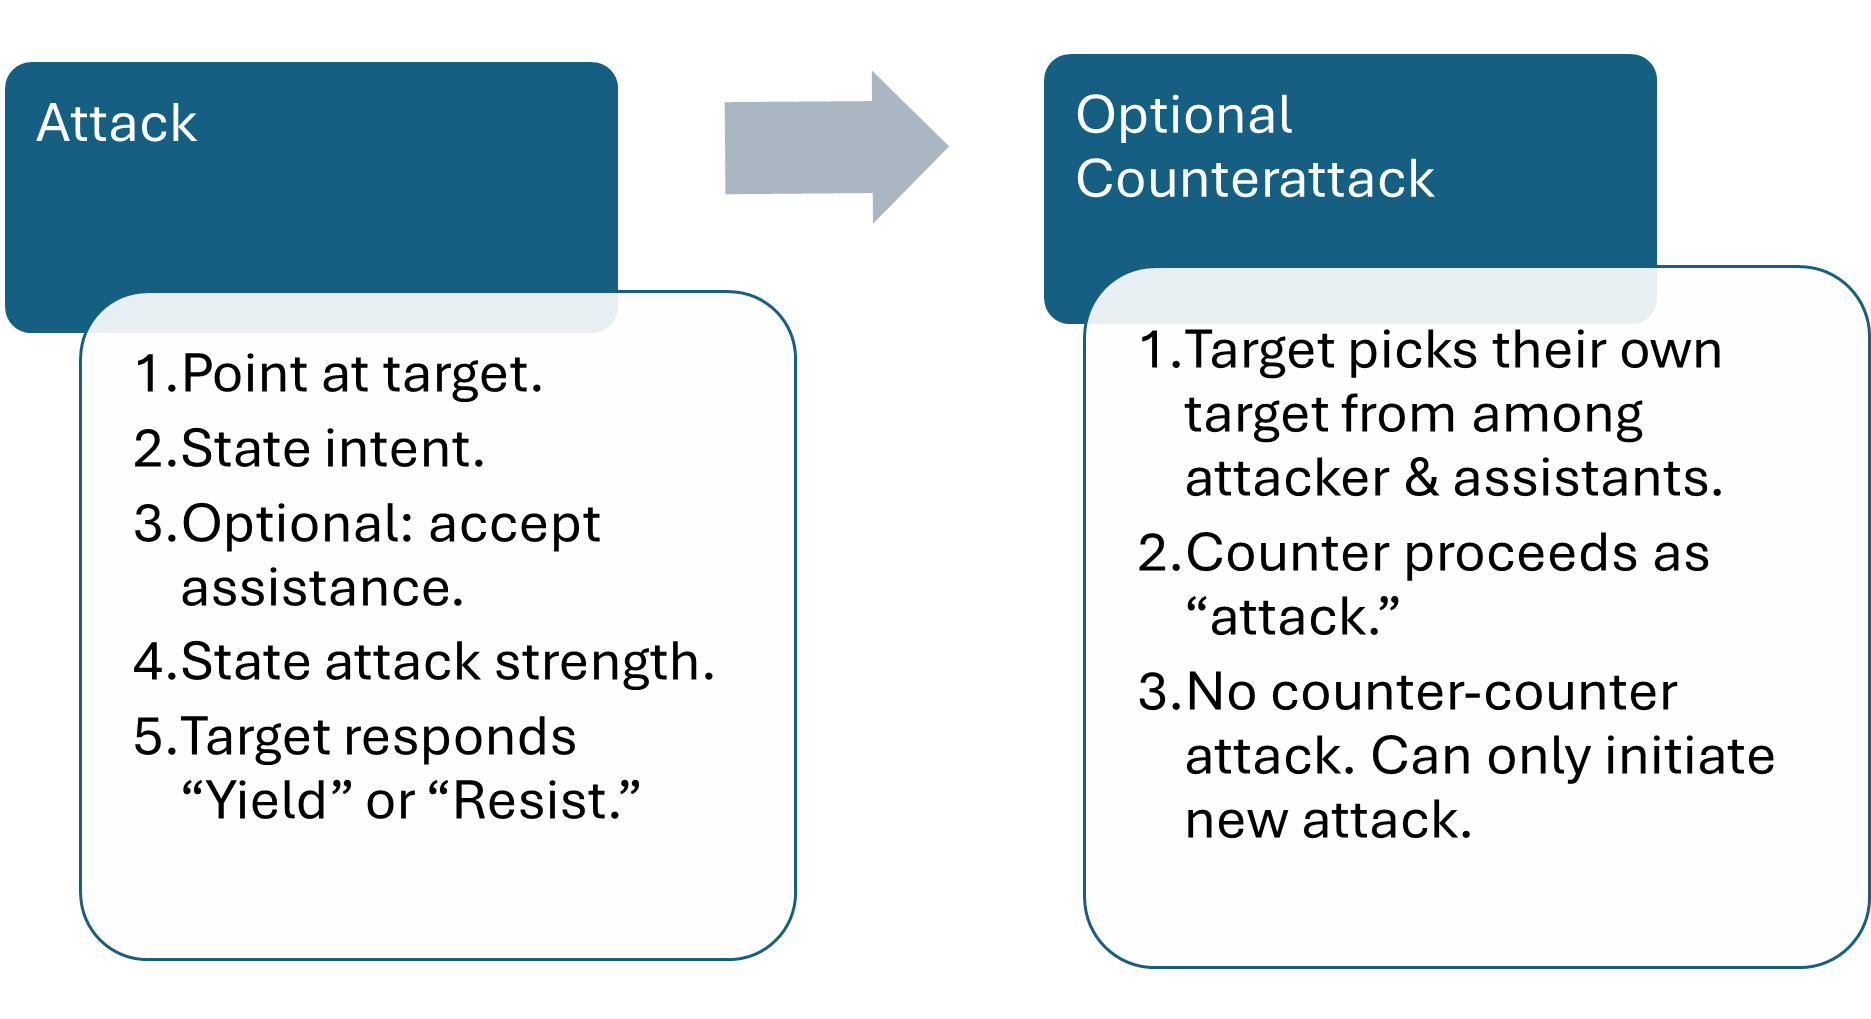
\includegraphics[width=0.8\textwidth]{\gamepath/images/CombatImage.png}
\end{center}

\paragraph{Cinematic Combat:} Once the Attacker's CR (plus any assists they choose to accept) has been compared to the Defender's CR, the Attacker can briefly narrate (in no more than a few words) what the attack looks like (i.e.: I throw a fireball at you.) If the defender is able to ``resist'’ they can briefly describe how the attack was dodged, parried, blocked, or otherwise nullified. If the defender cannot, or chooses not to resist, they should take the effect of the attack and may briefly describe how the attack affects them.

\textbf{Example:}\newline

Players 1, 2 and 3 want to Restrain player 4 so they can search Player 4’s bag. Players 1, 2 and 3 find Player 4 with just one other player, Player 5. Players 1-3 walk up within 1 Zone of Control to Player 4. Player 4 knows to be careful of these three, but is deep in conversation and does not see them coming.

\begin{enumerate}
	\item Player 1 has a CR of 3 and calls ``Resist'' points at Player 4, and waits briefly for any Assists.
 	\item Player 2 has a CR of 3 and decides to help, pointing at Player 1 and calling ``Assist 3.”
	\item Player 1 adds their own CR to Player 2’s CR for a total of 6, and completes their attack by calling ``6.''
	\item Player 3 decides to attempt to instead knock out Player 5 so that they don’t see what happens to Player 4. They state ``Knock Out,'' point at Player 5, and since there is no one with an action available to Assist, they state their CR, ``5.''
	\item Player 4 resolves the attack against them, comparing their own CR of 5 to the Restrain of 6. They can’t resist, given this, and Player 5 can’t help them defend. They state ``Yield.''
	\item Player 5 happens to have a high CR of 6. That is higher than the ``Knock Out 5'' directed against them by Player 4, so Player 5 says ``Resist.'' Note Player 5 should not state their CR out loud in order to Resist.
	\item Players 4 and 5 are both allowed counterattacks against their assailants, even though Player 4 failed to Resist the attack against them. For all intents and purposes, the counterattack is considered to be happening simultaneously with the original attack.
	\item For their counterattack, Player 4 points at Player 1, calls ``Knock Out,'' pauses briefly to see if Player 5 will assist (they choose not to), then finishes the attack by stating their CR of 5.
	\item Player 1's CR of 3 is lower than the ``Knock Out 5'' directed against them by Player 4, so they state ``Yield.''
	\item Player 5's counterattack is a Knock Out directed at Player 3; there is no one with an action available to Assist, so they state ``Knock Out 6,'' using just their own CR.
	\item Player 3's CR of 5 is lower than the ``Knock Out 6'' directed against them by Player 5, so they state ``Yield.''
	\item At this point, pause to describe what happens in a cinematic fashion. Players 1 and 3 are Knocked Out. The attack against Player 5 failed, so they are still conscious. Player 4 is restrained by Player 2 (who assisted the attack), because Player 1 is unconscious. Player 4 may not take any action while they are Restrained and Player 2 may not take any action while Restraining Player 4, but Player 5 is free to act. Combat may continue (Player 5 may declare ``Knock Out 6'' on Player 2, or Player 5 may run away to get help, leaving Player 4 helpless!). Note that in this example, none of Players 1, 2, or 3 end up in a position to actually search Player 4.
\end{enumerate}

\subsection{Stealth}

Stealth abilities represent sneaking up on a victim with obvious intent to invade their personal space, probably to attack them by surprise or to pick their pocket. Everyone has the ability to attempt a waylay attack (see below), but only some characters have additional stealth abilities.

To use a stealth ability, you must be within 1 ZoC of your victim. Form a ``llama'' with your hand (index and pinky fingers extended, thumb, middle and ring fingers touching) and extend it along the direct, unobstructed line from your shoulder to the victim's head. Hold this position for the time specified by your ability. Before this time is up, the ability is thwarted if anyone attacks you or if \textbf{anyone} declares that they notice the symbol. If your target reacts in any way to the symbol, they have noticed; you (the attacker) make the call if it is unclear. Any mechanic that requires a waylay is a suspicious activity, and characters who see you doing this may not think highly of it, or you.

If you notice someone using a stealth ability, make it obvious. ``I notice you'' or “I stop you” are unambiguous; use one of them if you can. Once a stealth ability is finished, you may not retroactively have noticed. You may choose \textbf{not} to declare notice of a waylay, for example if you are deliberately distracting the target so your friend can sneak up on them. 


\paragraph{Waylay Attacks:} Anyone can attempt to attack by surprise as a stealth ability. Even if you want to use a magical attack that allows for attacking from further away, waylay must always happen from within 1 ZoC. You must hold the symbol for a \textbf{5-count} (count silently: ``waylay 1’’, ``waylay 2’’, etc). If you succeed, you may replace your CR with ``waylay'' for a single immediate attack on your victim. If you are hit with a ``waylay attack'’, you do not have the opportunity to resist; you are surprised and the attack just works. (e.g. ``Upstage Waylay.’’ instead of ``Upstage 2’’. Unless you know otherwise, the only available response is ``yield.’’)


\textbf{Example:}\newline
Player One wants to sneak up behind player two and restrain them to take a relic that player two holds. Player One waits until Player Two is distracted by another conversation and comes up behind them. Player One makes the sign for waylay (the llama) behind Player Two and counts in their head for five seconds. Player Three notices Player One, but wants this to succeed so says nothing. Player One finishes the count and then declares “Restrain Waylay”. Player Two is now restrained and cannot resist the search.    


\subsection{Killing Blows and Character Death}

This weekend is a particular focus for the attention of the Gods. They will pay attention for as long as they can, until the growing power of the storm drives them away. \textbf{From Game Start until 9:00 pm on Saturday Night,} the attention of the Gods will make it impossible to kill anyone present at the \pSc{}. You may attempt to do so using the ``Killing Blow'' mechanic, but it will fail dramatically, even if you complete it successfully. You should feel free to roleplay this as impressively as you like. After 9:00 pm on Saturday night, the strength of the Storm will be too strong, and will drive the influence of the Gods far enough away for characters to be able to kill each other if they are willing to take the consequences.


\textbf{Unless you know otherwise, if you succeed in killing another character, your character will immediately lose all memory of who they are and what they were trying to accomplish.} Resolve any immediate roleplay in the scene, then ASAP, go to GM headquarters and take a copy of the appropriate information from the sign ``\sMurderConsequences{}''

The actual mechanic of a ``Killing Blow'' is an ``n-count'' of 10. To perform a killing blow: point at your target and incant ``killing blow 1,'’ ``killing blow 2,'’ etc. up to ``killing blow 10.'’ Speak loudly enough that anyone in the room with you could hear you, and slowly enough that each phrase takes at least 1 second. Anyone conscious and able to act within 1 ZoC of you may at any point before you reach ``10'’ say ``I stop you,'’ including your target if they are conscious. You are also interrupted if you are attacked. At which point, your character has been interrupted, and you must start over.

If your character is killed during game, \textbf{you MUST play the body for at least 10 minutes.} There may be some mechanics that utilize dead bodies.! After the 10 minutes has elapsed, leave your name badge on the ground to represent your body, and go OOC (fist on head). Go to the GM HQ and take a greensheet from the sign ``\sMurdered{}''

\textbf{Example:}\newline
It is Sunday morning and Player 1 has discovered that Player 2 killed their family! Player One knows the consequence but feels they must act. Player 1 comes up to Player 2 when they are alone. 
\begin{enumerate}
	\item Player 1: Declares an attack: ``Knockout 5.'' 
	\item Player 2: They have only CR 4 and no one near them. They state ``Yield.''
	\item Player 1: While Player 2 is knocked out they start the killing blow count, out loud (``Killing Blow One, Killing Blow Two,\ldots'')
	\item As Player 1 counts, Player 3 comes around the corner and overhears what Player 1 is saying. Player 3 states loudly ``I stop you'' before Player 1reaches ``Killing Blow Ten.'' At this point, Player 1 must stop their killing blow. They can try and start it again, but it is likely that Player 3 will keep stopping them. If Player 2 wants to get rid of Player 3, they may need to also attack Player 3 at this point.
\end{enumerate}

\section{Miscellaneous}

\paragraph{Badge Numbers:} The first digit of your badge number is your character's apparent age in decades.

\subsection{Changing Patrons or Abandoning the Gods:}
If your character wishes to change Patron Gods, speak to a Cleric of that Patron. If your character wishes to abandon \textbf{all} of the gods, and attempt to live without a patron, speak to a GM.

\subsection{Magic:}
{Magic is everywhere in this game. All combat is magic. Curses are magic. Building technology that works is magic. Growing food is magic. The avatars of the Deities are magic. Most of your abilities are powered by magic either overtly or subtly. The voting stones are magic. The Relics are magic. And all of the rituals in game represent groups casting magic together.

\subsubsection{Recovering CR:}
Some mechanics will temporarily reduce your CR. Keep track of this by discarding a CR stone to the nearest stock, or do whatever the mechanic says to do with the stone. For future CR checks, your CR is whatever your current number of stones is.

\textbf{At the next meal,} draw stones back up to your maximum (the number printed on your character sheet). There are only a very small number of mechanics that will change your maximum, and will say so explicitly.

\subsubsection{Rituals:}
Many characters have rituals they wish to accomplish in game. Expect to need to teach/guide your fellow participants how to execute your ritual. Use this as a roleplay opportunity. Please also make it clear to participants and onlookers when a ritual is \textbf{finished} as that may not be obvious.

\subsubsection{Relic Attunement:}
The Relics can do incredible things, but only as long as they are ``attuned’’ to a location. Which location does not matter, but they must be attuned. Unless a mechanic explicitly says otherwise, \textbf{any} use of a Relic, either for its innate ability, or for something else will ``de-attune’’ the Relic. \textbf{Clerics know how to re-attune Relics, as well as how to check what the current attunement is.}

To check if a Relic is currently attuned to someplace, open the attached envelope and see if there is a piece of paper inside \textbf{DO NOT} pull the paper out and read it! You will need to do this to verify if you can in fact use the Relic for a mechanic that requires it to be attuned. If there is no paper inside, the Relic is not attuned, and cannot be used for a mechanic that requires it to be attuned.

To de-attune a Relic, open up the envelope, withdraw the piece of paper, and discard it to the nearest stock or hand it to the nearest GM. \textbf{DO NOT} read the piece of paper. You don’t get to learn where the Relic \emph{was} attuned before the attunement got used up. Relics can only be de-attuned by using them for a mechanic that calls for it. You cannot just de-attune a Relic; de-attunement represents the energy of the Relic being transferred to another magical effect.

Relics can be attuned to any location, not just to the nation they are typically associated with.

\subsubsection{Curses:}
Some characters have the ability to create curses (and cures for those curses, but ``curse'' is the umbrella term). These are represented by item cards or item-envelopes that describe their effects. Some curses will have associated abilities or greensheets. Curses begin as latent magical effects, but can be activated in one of several ways. Once activated, write ``expended'' on the card and the person upon whom the curse is active should carry it around with them to remind themselves of the effect until it ends. ``Expended'' curses no longer represent physical items, they are just OOC reminders.

\subsubsection{Activating a Curse:}
Unless you know otherwise, you may:
\begin{itemize}
	\item Choose to activate a curse on yourself, as long as you are not unconscious or restrained.
	\item Activate a curse on a willing target. 
	\item Activate a curse on an unconscious, restrained, or upstaged target.
	\item Use a waylay with a 5-count to secretly activate a curse on someone. (Hand the item to a GM. We will pass it on to your target as quickly as we can while avoiding casting suspicion on you. You may even hand the curse to a GM preemptively if you are about to attempt the waylay.)
	\item Some mechanics may specify other ways to activate a specific curse on someone.
\end{itemize}

Some curses may specify more stringent requirements for activation. Such items will say so. e.g. ``you cannot activate this curse unless you know otherwise.'' See a GM if you have any questions.

\subsubsection{Maker's Marks:}
Every magic user has a unique signature to their magic. For the purposes of game, this is most relevant regarding the construction of curses. Every curse will have a maker's mark on it. These marks are only visible and interpretable to Advanced Cursemakers. To everyone else, the marks mean nothing and should be considered out of game information and ignored. 

\subsection{Randomization Mechanics:}
Several mechanics in this game use D20 dice for a randomization mechanic. The GMs will have D20s available for your use during game (and to keep afterwards.) You will want to keep this die handy as it may be called for at unexpected times.

\subsection{Colored Tape:}
Masking tape of \textbf{any color} that is stuck to a wall, floor, tarp/carpet, etc CANNOT be removed unless you know otherwise. This tape represents some sort of \textbf{in game} effect. You should look around for a sign nearby that explains what is being represented.

\subsection{In Game Mail:}
Anyone may write letters to people and send them off, but you won't get a response, and there is no guarantee that such letters will reach their intended destination. Some characters have the ability to send mail out to specific entities, and expect a response before the weekend ends. For those characters, GMs will distribute responses at each meal. 

\subsection{Drawing Blood:}
Some mechanics may call for drawing blood or acquiring a blood sample. \textbf{This is not a free action.} You \textbf{must} have a suitable vessel to contain the sample — if your character does not start with knowledge of which items can hold blood, you will need to either search gamespace, or ask around, until you find one. \textbf{Further,} you may only actually draw the blood in a location or with an item that says ``you could cut yourself here'' or something to similar effect. \emph{OOC Note: there are no descriptions of needles in game, and absolutely NO phys reps of needles. All mentions of blood are brief and non-graphic.} You can draw blood from yourself, or a willing or helpless (restrained or unconscious) target.

\subsection{Storing Items:}
As a reminder: An object may be bulky, unstashable, have a prop, or any combination of all 3. If the prop and the item card get separated, the \textbf{item card} is the real instance. Bulky items have to be carried visibly. Unstashable items cannot be physically hidden in the environment (though they can be hidden on a person). \textbf{NO} items can be put into envelopes unless a mechanic specifically says you can do so for that particular item and/or that particular location.

\subsection{Consuming Items:}
As a reminder: Unless you know otherwise, items, whitesheets, etc. \textbf{cannot be destroyed}. This is a kludge. Some mechanics will involve ``consuming'' items. \textbf{Please discard these items to the nearest stock vessel (or give them to the nearest GM) rather than tearing them up or throwing them away.} This will save time and paper for items that are unlimited for the purposes of game without us having to print a thousand copies just in case.}

\subsection{The Library:}
The vast, labyrinthine Library of the College of the Gods is represented in game by a choose-your-own adventure booklet, of which there will be numerous copies. The first page of the booklet lays out the rules for exploring the Library. They are also below should you wish to review them before game:

\begin{enumerate}
	\item When you turn to a page, read the list of options, pick one, and follow its instructions. If you remain on that page, you can then pick another option. Repeat on the next page you turn to. \textbf{You cannot backtrack to a location you just came from unless there is an option to do so in the text.}
	\item You may explore the Library in a group as long as there is consensus on all decisions made. If there is disagreement, you must proceed separately. If you encounter another group at the same location (by comparing notes \textbf{OOC} and realizing you are in the same place), you are welcome to merge.
	\item Some options require that certain conditions be met (e.g. a CR threshold). As long as anyone in your group meets the condition, the whole group may take that option (\textbf{unless} the text states otherwise); for meeting CR thresholds, count everyone’s CR \textbf{combined}, then \textbf{add} the highest L-Score in your group. 
	\item Some options ask you to roll a d20; high rolls are usually more favorable. 
	\item Some options let you interact with one of the envelopes located here. Do not remove items from or place items in these envelopes unless instructed to do so. If you wish to leave an item at any location in the Library where you are not instructed to do so, place it in “Envelope 14: Lost and Found.” \textbf{Even items which are normally “Unstashable”} can be placed in “Envelope 14: Lost and Found.”
	\item The Library is dangerous, especially the deeper levels. You may be injured, Cursed, forced to drop items, faced with existential horror, or separated from your group. All effects are \textbf{temporary}, with one signposted \& avoidable exception. Traveling in groups \& with people who have high L-Scores is safer.
	\item You can gain certain status effects in the Library, such as a “Memory of Light” or a “Flash of Inspiration.” The Library text will tell you when and where these have any mechanical effect and what that effect is. \textbf{Unless} the text states otherwise, all status effects expire when you leave the Library.
	\item You can conduct research in the Library by finding a Catalog; the deeper you go, the more esoteric questions you can ask. You cannot use Library research to do an “end run” around a research notebook or greensheet, though you may get a hint.
	\item If you want to interact with the Library in a way that isn’t listed among the options, find a GM.
	\item At any time, you may Flee Blindly from the Library, which lets you exit the Library immediately, regardless of location. First, however, you \textbf{must return} any items you obtained in the Library to their original envelopes as you drop them in panic. \textbf{Each} person who has no such items to drop must instead draw a \textbf{random} Curse from “Envelope 3: Cursed Codices;” they are now affected by the Curse they drew. Read the Curse, then put it back in the envelope. You \textbf{may not return} to the Library until everyone's Curses have worn off. 
\end{enumerate}

\section{Closing Notes}

These rules are imperfect. The GMs may violate the letter of the rules to preserve the spirit. We hope these rules are reasonably clear, but if you have any doubts about your interpretation, talk it over with us in advance. We GMs are human too: When all of our carefully laid plans are going haywire, we may lose our cool. The best way to deal with people is remaining calm and friendly, especially if everyone is tired and hungry.

We hope you have lots of fun. Good luck.

\end{document}
